\newpage
\section{Getting Started}
The University Management systems has been created using Java, this means that in order to run the program, there needs to exist a class that allows for the program for the program to run. In the UMS, we designed the loginScreen class as the program to run, once the user runs the loginScreen class it will begin the program.

The ability to run the software requires the installation of IntellJ or Replit, or another IDE that allows Java programs to run functionality. It is important to note that the University Management System is subject to version changes or updates to Java. For more details relating to the code, refer to the Class Library for each of the classes that were designed. Once the user runs the program through IntellJ by running the Login Screen class, begin by entering the correct credentials provided by the University of Guelph, see \autoref{fig:example1}


\begin{figure}[ht]
    \centering
        \centering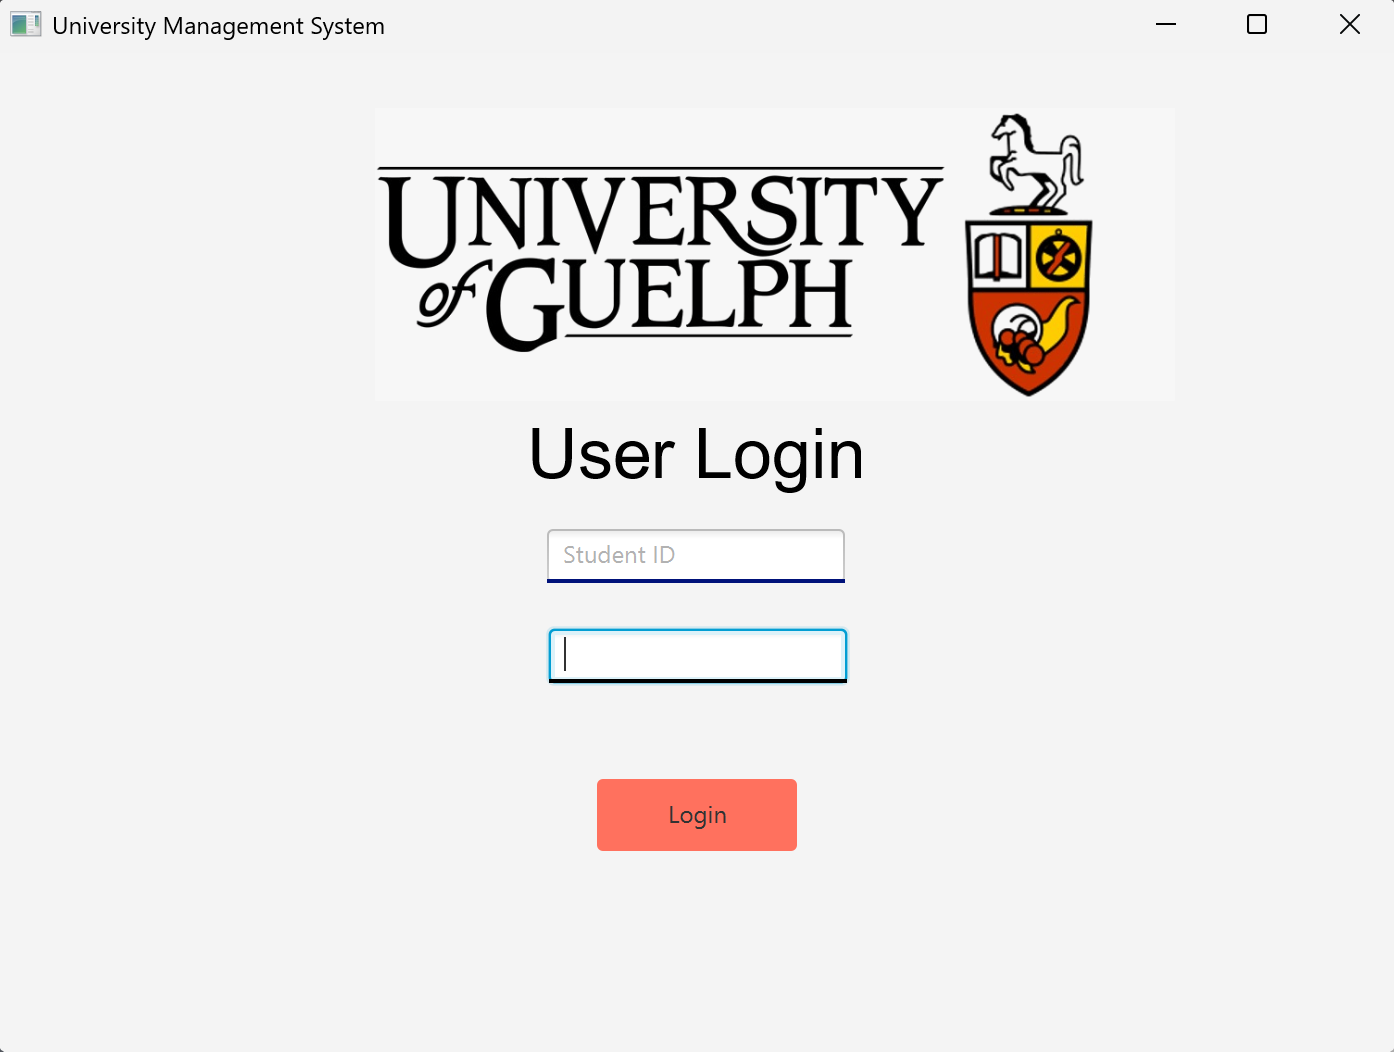
\includegraphics[width=1\linewidth]{figures/login_screen.png}
        \caption{Login Screen}
        \label{fig:example1}  
\end{figure}

% \subsection{Password Recovery (Optional)}


\subsection{First-Time Login Guide}

Once the user is at the login screen after running the program, they have either three login options to utilize the UMS program; faculty, student, and administrator. Each of these log-in credentials provides specific privileges that allow for editing such as deleting or adding, viewing, or changing personal settings. First time users must provide their correct login information in order to access the system, if they enter either an incorrect password or incorrect username, the user will receive an error message (see \autoref{fig:example2} below). This error will continue to occur until the user places the correct information, the user must login with the correct username and password; otherwise, it will continue to provide an error.


\begin{figure}[ht]
    \centering
        \centering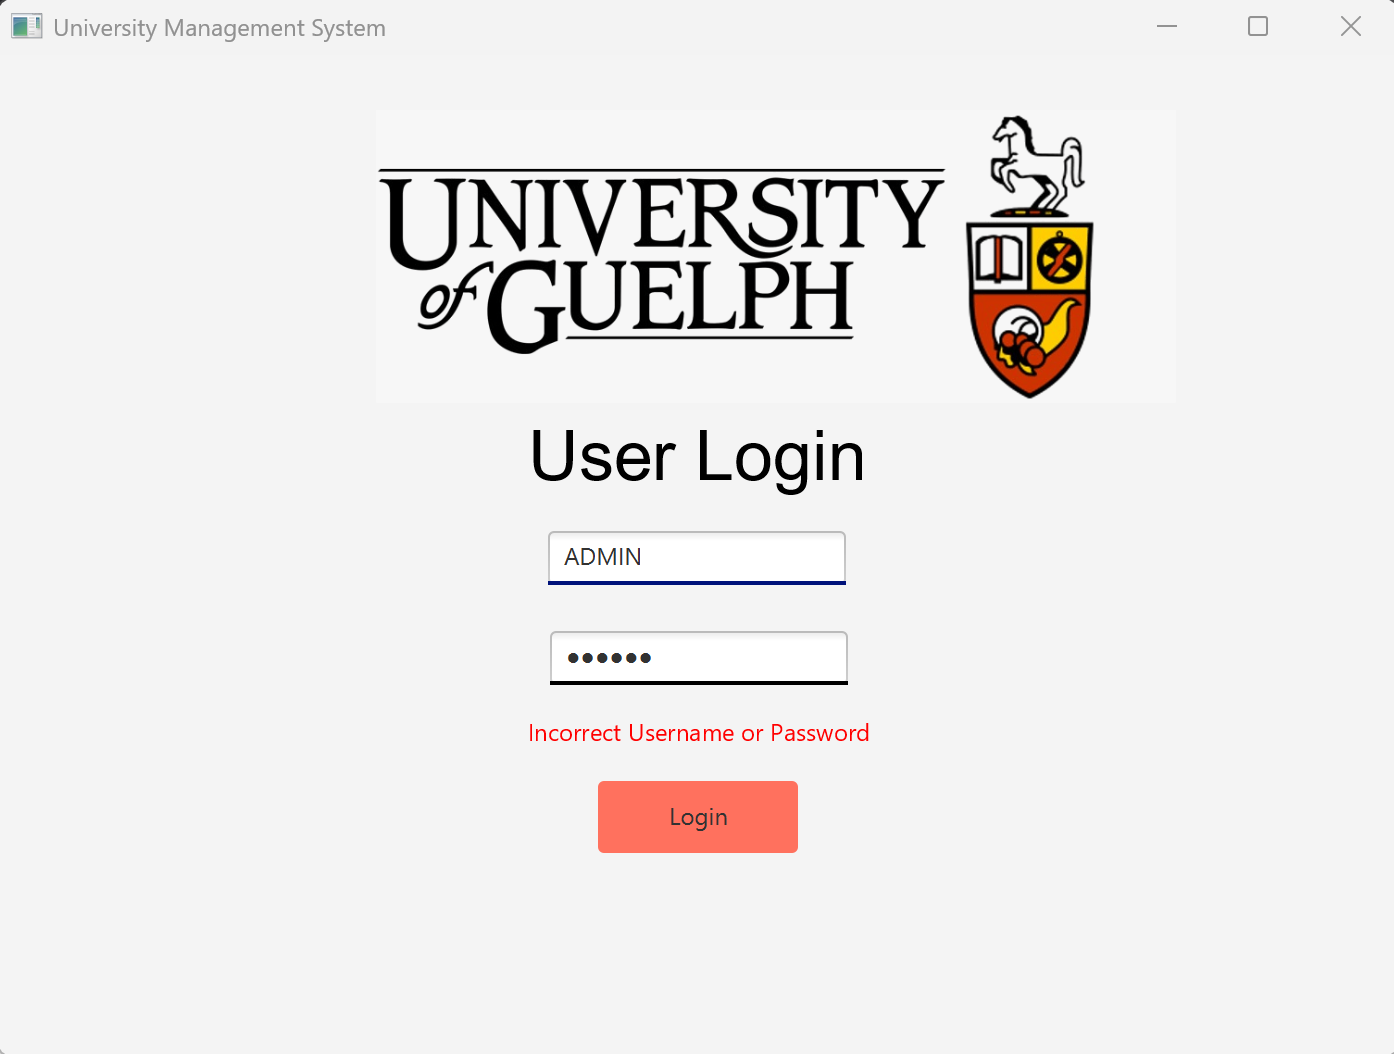
\includegraphics[width=1\linewidth]{figures/Incorrect_PW.png}
        \caption{Invalid Username/Password}
        \label{fig:example2}  
\end{figure}